\enteteThematiqueObligatoire{}
\enteteCorrection{}

%%%%%%%%%%%%%%%%%%%%%%%%%%%%%%%%%%%%%%%%%%%%%%%%%%%%%%%%%%%%%%%%%%%%%%%%%%
\encadreTDExo{1 - Montage transimpédance - Etude simple}{
\begin{itemize}[label=$\triangleright$,leftmargin=*]
	\item Modélisation d'une photodiode et d'un oscilloscope
	\item Intérêt de l'ALI pour un système de photodétection
\end{itemize}
}

On considère le montage récepteur à photodiode suivant. L'amplificateur linéaire intégré (ALI) est alimenté en $\pm15\operatorname{V}$. On note $\Phi_{lum}(t)$ le flux lumineux reçu par la photodiode et $k$ sa sensibilité.

\begin{figure}[!h]
\centering
\begin{circuitikz} 
	\node [op amp](A1) at (0,0){\texttt{ALI1}};
	\draw (A1.-) to[short] ++(-.5,0) coordinate(A) to[short] ++(0,1.5) coordinate(B) to[R=$R_F$, i=$i_R$] (B -| A1.out) to[short, -*] (A1.out);
	\draw (A1.- -| -5,0) node[ground]{};
	\draw (A1.- -| -5,0) to[I, invert, i=$i_{Phd}$, *-*] (A);
	\draw (A1.- -| -5,0) -- ++(0,1.5) to[C, l=$C_{Phd}$, i=$i_C$, -*] (B);
	\draw (A1.+) to[short] ++(0,-0.5) node[ground]{};
	\draw (A1.out) -- ++(1,0) coordinate(D);
	\draw (2.2,-2.1) edge[->, color={red}] (2.2,-0.3);
	\node[text={red}] (Vs) at (1.7,-1.2){$V_s$}; 
	\draw (D) -- ++(1,0) to[C,l=$C_{e}$, *-*] ++(0,-2.5) coordinate(G);
	\draw (G) node[ground]{};
	\draw (G) -- ++(2,0) to[R,l=$R_e$] ++(0,2.5) -- ++(-2,0);
\end{circuitikz}
\end{figure}

\begin{enumerate}
	\item A quoi correspondent les différents éléments de ce montage ?
\answer{
	$C_{Phd}$ correspond à la capacité de jonction de la photodiode.
	
	$R_e$ et $C_e$ correspondent à l'impédance d'entrée de l'instrument de mesure du signal $V_S$ (un oscilloscope par exemple) et à la capacité des câbles permettant d'amener le signal vers l'appareil de mesure.
}
	\item Dans quel mode de fonctionnement est l'ALI ?
\answer{
	Il y a une contre-réaction négative, l'ALI fonctionne donc en mode linéaire. On peut ainsi dire que $V+=V-$.
}
	
	\item Exprimez la tension de sortie $V_S(f)$ en fonction de $i_{Phd}$ et des éléments du montage. 

\answer{
	Comme $V^+ = V^-$, la photodiode est donc polarisée avec une tension constante et la capacité se retrouve avec une différence de potentiel constante à ses bornes, ainsi $i_c = 0$. 

	On a donc : $V_S(f) = - R_F \cdot i_{Phd}$.

	Mais cette représentation ne permet pas de décrire les résultats expérimentaux obtenus, à savoir : une résonance dans la réponse en fréquence et un comportement passe-bas.
}
\end{enumerate}

%%%%%%%%%%%%%%%%%%%%%%%%%%%%%%%%%%%%%%%%%%%%%%%%%%%%%%%%%%%%%%%%%%%%%%%%%%
\encadreTDExo{2 - Montage de contre-réaction}{
\begin{itemize}[label=$\triangleright$,leftmargin=*]
	\item Filtre linéaire
\end{itemize}
}

On étudie le montage suivant :

\begin{figure}[!h]
\centering
\begin{circuitikz}
	\draw (0,0) to[I,i=$i_{Phd}$,*-] (0,3) -- (2,3) -- (3,3) to[R,l=$R_F$, i=$i_R$] (5,3) to[short, -o] ++(0.5,0);
	\draw (0,0) -- (2,0) to[C,l=$C_{Phd}$,*-*, i=$i_C$] (2,3);
	\draw (2,0) -- (5,0) to[short, -o] ++(0.5,0);
	% fleches
	\draw (2.8,0.3) edge[->, green!40!black] (2.8,2.7); \node[text=green!40!black] (U-) at (3.2,1.5){$V-$};
	\draw (5.5,0.3) edge[->, red!40!black] (5.5,2.7); \node[text=red!40!black] (U-) at (5.9,1.5){$V_S$};
	\draw (0,0) node[ground](GND){};
\end{circuitikz}
\end{figure}

\begin{enumerate}
	\item Calculez les courants $i_R$ et $i_C$ en fonction des éléments du montage.
\answer{
	$$i_R = \frac{V^- - V_S}{R_F}$$
	
	$$i_C = - \frac{V^-}{\frac{1}{j \cdot C \cdot \omega}}$$
}
	\item Quel est le lien entre $i_R$, $i_C$ et $i_{Phd}$ ?
\answer{
	Par la loi des noeuds, $i_{Phd} + i_C - i_R = 0$.
}
	\item Que vaut alors $V^-$ en fonction de $V_S$ et $i_{Phd}$ ?
\answer{
	On obtient :
	
	$$i_{Phd} + \frac{V_S}{R_F} - \frac{V^-}{R_F} - V^- \cdot j \cdot C_{Phd} \cdot \omega = 0$$
	
	Ce qui donne :
	
	$$V^- = (V_S + R_F \cdot i_{Phd}) \cdot \frac{1}{1 + j \cdot R_F \cdot C_{Phd} \cdot \omega}$$
}
	\item Dans le cas où $i_{Phd} = 0$, quel est le comportement en fréquence du système entre $V_S$ et $V^-$ ?
\answer{
	D'après la relation précédente :
	$$\frac{V^-}{V_S} = \frac{1}{1 + j \cdot R_F \cdot C_{Phd} \cdot \omega}$$
	
	Il s'agit d'un filtre passe-bas de fréquence de coupure $f_c = \frac{1}{2 \cdot \pi \cdot R_F \cdot C_{Phd}}$.
}
\end{enumerate}

%%%%%%%%%%%%%%%%%%%%%%%%%%%%%%%%%%%%%%%%%%%%%%%%%%%%%%%%%%%%%%%%%%%%%%%%%%
\encadreTDExo{3 - Transimpédance et modèle du premier ordre pour l'ALI}{
\begin{itemize}[label=$\triangleright$,leftmargin=*]
	\item Modèle de l'ALI du premier ordre
	\item Système linéaire
\end{itemize}
}

Soit le montage suivant :

\begin{figure}[!h]
\centering
\begin{circuitikz} 
	\node [op amp](A1) at (0,0){\texttt{ALI1}};
	\draw (A1.-) to[short] ++(-.5,0) coordinate(A) to[short] ++(0,1.5) coordinate(B) to[R=$R_F$, i=$i_R$] (B -| A1.out) to[short, -*] (A1.out);
	\draw (-5,-1.6) edge[->, color={blue}] (-5,0.2);
	\node[text={blue}] (VR) at (-4.5,-0.7){$V_R$};
	\draw (-5, -1.8) to[short, o-] ++(0,0.1) node[ground]{};
	\draw (A1.- -| -5,0) to[I, invert, i=$i_{Phd}$, *-*] (A);
	\draw (A1.- -| -5,0) -- ++(0,1.5) to[C, l=$C_{Phd}$, i=$i_C$, -*] (B);
	\draw (A1.+) to[short] ++(0,-0.5) node[ground]{};
	\draw (A1.out) -- ++(1,0) coordinate(D);
	\draw (2.2,-2.1) edge[->, color={red}] (2.2,-0.3);
	\node[text={red}] (Vs) at (1.7,-1.2){$V_s$};
	\draw (2.2, -2.4) to[short, o-] ++(0,0.1) node[ground]{}; 
\end{circuitikz}
\end{figure}

On modélisera l'ALI par son modèle du premier ordre :

$$A(j \cdot \omega) = \frac{A_0}{1 + \frac{j \cdot \omega}{\omega_0}}$$

où $A_0$ est l'amplification différentielle statique et $\omega_0 = \frac{GBP}{A_0}$ la pulsation de coupure, avec $GBP$ la bande-passante unitaire.

\begin{enumerate}
	\item Que vaut $V_S$ en fonction de $V^+$ et $V^-$ ?
\answer{
	$V_S = A(p) \cdot (V^+ - V^-)$
}
	\item Quel est le lien avec le montage de l'exercice 2 ?
\answer{Le montage de l'exercice 2 se retrouve dans la contre-réaction du montage transimpédance.}
	\item Que vaut alors $V_S$ en fonction de $i_{Phd}$ ?
\answer{
	$V^+ = 0$ et $V^-$ est la relation trouvée à la fin de l'exercice 2.
	
	On alors :
	
	$$V_S = - A(j \cdot \omega) \cdot (V_S + R_F \cdot i_{Phd}) \cdot \frac{1}{1 + j \cdot R_F \cdot C_{Phd} \cdot \omega}$$
	
	Ce qui donne :
	
	$$V_S \cdot (1 + A(j \cdot \omega)) \cdot \frac{1}{1 + j \cdot R_F \cdot C_{Phd} \cdot \omega} = - R_F \cdot i_{Phd} \cdot \frac{1}{1 + j \cdot R_F \cdot C_{Phd} \cdot \omega}$$
	}
	
	On notera $\omega_c = \frac{1}{R_F \cdot C_{Phd}}$ et $K = \frac{A_0}{1 + A_0}$.
	
	\item Quelle est la fonction de transfert de ce montage ?
\answer{
	$$\frac{V_S}{i_{Phd}} = - A(j \cdot \omega) \cdot \frac{R_F}{1 + j \cdot R_F \cdot C_{Phd} \cdot \omega}$$	
	
	En développant, on obtient : 
	
	$$\frac{V_S}{i_{Phd}} = - \frac{A_0 \cdot R_F}{1 + A_0 + j \cdot \omega \cdot (\frac{1}{\omega_c} + \frac{1}{\omega_0}) + (j \cdot \omega)^2 \cdot \frac{1}{\omega_c \cdot \omega_0}}$$
	
	On obtient au final :
	
	$$\frac{V_S}{i_{Phd}} = - K \cdot \frac{R_F}{1 + j \cdot \omega \cdot \frac{K}{A_0} (\frac{1}{\omega_c} + \frac{1}{\omega_0}) + (j \cdot \omega)^2 \cdot \frac{K}{A_0} \frac{1}{\omega_c \cdot \omega_0}}$$	
	
	Ou
	
	$$\frac{V_S}{i_{Phd}} = - K \cdot \frac{R_F}{1 + j \cdot \omega \cdot \frac{1}{1 + A_0} (\frac{\omega_c + \omega_0}{\omega_c \cdot \omega_0}) + (j \cdot \omega)^2 \cdot \frac{1}{1 + A_0} \frac{1}{\omega_c \cdot \omega_0}}$$
}
	\item Calculez les valeurs de la pulsation propre $\omega_T$, le facteur d'amortissement $m_T$ et le gain statique $G_T$ de ce système.
\answer{
	Ce système est un système du second ordre, de type passe-bas.
	
	$$G_T = K \cdot R_F$$
	
	$$\omega_T = \sqrt{(1 + A_0) \cdot \omega_c \cdot \omega_0}$$
	
	$$m_T = \frac{\omega_T}{(1 + A_0) \cdot \omega_c \cdot \omega_0} \cdot \frac{\omega_c + \omega_0}{2}$$
}
	\item Que deviennent ces valeurs si on suppose que $A_0 >> 1$ ?
\answer{
	On a : $K \approx 1$
	
	Et ainsi : $G_T \approx R_F$
	
	$$\omega_T \approx \sqrt{\omega_c \cdot A_0 \cdot \omega_0} = \sqrt{\omega_c \cdot \omega_{GBP}}$$
	
	$$m_T = \frac{\omega_c + \omega_0}{2 \cdot \omega_T} \approx \frac{1}{2} \cdot \sqrt{\frac{\omega_c}{\omega_{GBP}}}$$
}

	On prendra les valeurs suivantes pour la suite :
	
	$A_0 = 2 \cdot 10^5$, $GBP = 3\operatorname{MHz}$, $R_F = 100\operatorname{k\Omega}$ et une photodiode de type SFH206 (dont une courbe caractéristique est donnée ci-après).
	
\begin{figure}[!h]
	\centering
	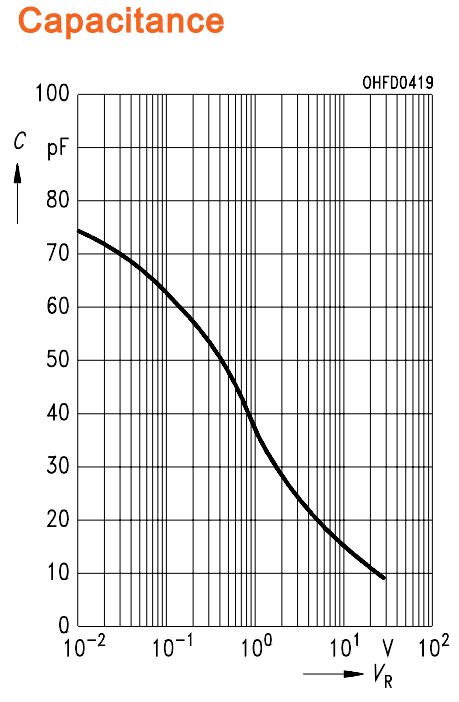
\includegraphics[width=6cm]{images/TD/SFH206_capa.png}
\end{figure}
	
	\item Que valent $\omega_T$ et $m_T$ pour $V_R = 0\operatorname{V}$ ? Pour $V_R = 30\operatorname{V}$ ?
\answer{
	Pour $V_R = 0\operatorname{V}$, on a $C_{Phd} = 75\operatorname{pF}$.
	
	On a alors : $\omega_c = 133.3\operatorname{krd/s}$ ($f_c = 21.2\operatorname{kHz}$), $\omega_T = 1.58\operatorname{Mrd/s}$ ($f_T = 252\operatorname{kHz}$) et $m_T = 0.04$.
	
	\medskip
	
	Pour $V_R = 30\operatorname{V}$, on a $C_{Phd} = 10\operatorname{pF}$.
	
	On a alors : $\omega_c = 1\operatorname{Mrd/s}$ ($f_c = 159\operatorname{kHz}$), $\omega_T = 4.34\operatorname{Mrd/s}$ ($f_T = 690\operatorname{kHz}$) et $m_T = 0.115$.
	
}
	
	\item Quelles formes ont les réponses en fréquence pour ces deux valeurs de tension de polarisation ?
\answer{
	Réponse en fréquence d'un second ordre avec résonnance.
	\begin{center}
	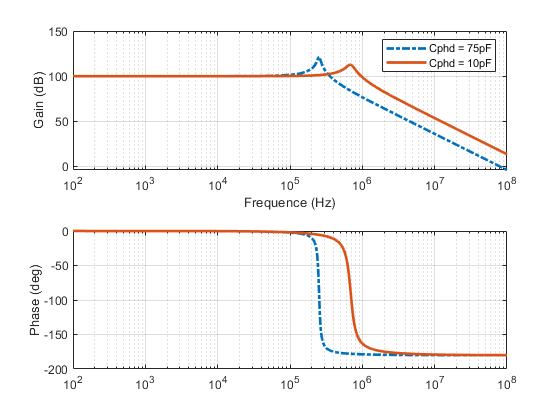
\includegraphics[width=10cm]{images/TD/Bode_sys_corr.png}
	\end{center}
	
}
	
	\item Parmi les deux réponses indicielles suivantes, laquelle est celle pour $V_R = 0\operatorname{V}$ ? Pour $V_R = 30\operatorname{V}$ ?
\begin{figure}[!h]
	\centering
	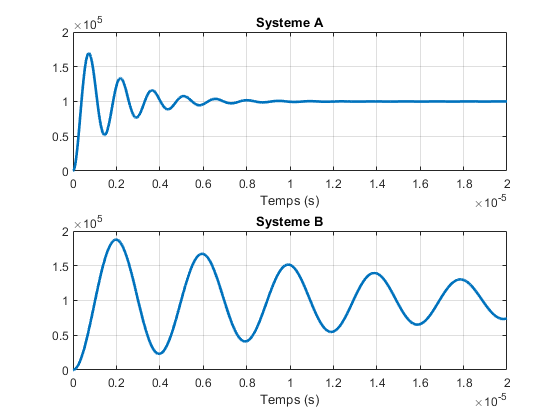
\includegraphics[width=10cm]{images/TD/step_sys.png}
\end{figure}
\answer{
	Le système A correspond à un facteur d'amortissement plus important que le système B.
	
	On peut donc supposer que le système A correspond à $V_R = 30\operatorname{V}$ et le système B à $V_R = 0\operatorname{V}$.
	
	On pourrait aussi comparer les fréquences des oscillations. Celle du système A est plus grande que le système B. Cela concorde également avec la réponse précédente.
}

\end{enumerate}
